\documentclass[letterpaper,10pt]{article}

\usepackage{titling}
\usepackage{listings}
\usepackage{url}
\usepackage{setspace}
\usepackage{subfig}
\usepackage{sectsty}
\usepackage{pdfpages}
\usepackage{colortbl}
\usepackage{multirow}
\usepackage{multicol}
\usepackage{relsize}
\usepackage{amsmath}
\usepackage{wasysym}
\usepackage{fancyvrb}
\usepackage{amssymb}
\usepackage{ifsym}
\usepackage{amsmath,amssymb,amsthm,graphicx,xspace}
\usepackage[titlenotnumbered,noend,noline]{algorithm2e}
\usepackage[compact]{titlesec}
\usepackage{XCharter}
\usepackage[T1]{fontenc}
\usepackage{tikz}
\usetikzlibrary{arrows,automata,shapes,trees,matrix,chains,scopes,positioning,calc}
\tikzstyle{block} = [rectangle, draw, fill=blue!20, 
    text width=2.5em, text centered, rounded corners, minimum height=2em]
\tikzstyle{bw} = [rectangle, draw, fill=blue!20, 
    text width=4em, text centered, rounded corners, minimum height=2em]

\definecolor{namerow}{cmyk}{.40,.40,.40,.40}
\definecolor{namecol}{cmyk}{.40,.40,.40,.40}

\let\LaTeXtitle\title
\renewcommand{\title}[1]{\LaTeXtitle{\textsf{#1}}}


\newcommand{\handout}[5]{
  \noindent
  \begin{center}
  \framebox{
    \vbox{
      \hbox to 5.78in { {\bf ECE356: Database Systems } \hfill #2 }
      \vspace{4mm}
      \hbox to 5.78in { {\Large \hfill #4  \hfill} }
      \vspace{2mm}
      \hbox to 5.78in { {\em #3 \hfill} }
    }
  }
  \end{center}
  \vspace*{4mm}
}

\newcommand{\lecture}[3]{\handout{#1}{#2}{#3}{Lecture #1}}
\newcommand{\tuple}[1]{\ensuremath{\left\langle #1 \right\rangle}\xspace}

\addtolength{\oddsidemargin}{-1.000in}
\addtolength{\evensidemargin}{-0.500in}
\addtolength{\textwidth}{2.0in}
\addtolength{\topmargin}{-1.000in}
\addtolength{\textheight}{1.75in}
\addtolength{\parskip}{\baselineskip}
\setlength{\parindent}{0in}
\renewcommand{\baselinestretch}{1.5}
\newcommand{\term}{Winter 2018}

\singlespace


\begin{document}

\lecture{ 31 --- Parallel Databases }{\term}{Jeff Zarnett}

\section*{Parallelism in Databases}

Although this is not a course on concurrency, parallelism, and synchronization, we will take some small amount of time to discuss how these impact on database implementation.  Let's assume that we have a multicore system available because, let's face it, it's not 1999 anymore.

The first way that we could achieve parallelism or concurrency is based on how we decide to implement the server. If each incoming transaction to be processes is assigned a thread, then we could have $n$ worker threads and a transaction gets picked up by a worker. Keeping in mind that locking and coordination are needed, but the maximum theoretical speedup is limited by the number of processors. Alternatively there could be a more segmented approach where rather than a worker that takes a job from start to finish there are different ``segments'' of a pipeline and those run in parallel. But that sort of thing is what we have covered in previous discussions. 


\subsection*{I/O Parallelism} If the database is aware of the various disks available in the system, we can speed up performance via I/O parallelism. If we need to read some blocks from disk, we could let multiple requests run in parallel. If there are three blocks we need, and three disks, we could get all three results at (roughly) the same time. 

We'll consider three basic partitioning strategies assuming we have $n$ disks available~\cite{dsc}:
\begin{itemize}
	\item \textbf{Round-Robin}: When data is being written, the $i$th tuple is sent to disk $i$ modulo $n$. This gives very even distribution of tuples.
	\item \textbf{Hash Partitioning}: Each tuple is passed through some hash function that produces a result in the range $[0, n-1]$ and each tuple of the relation is sent to the disk that matches the hash function.
	\item \textbf{Range Partitioning}: Assigns ranges of tuples to various disks. For example, is the values can be A, B, C, or D and there are two disks, we might assign A and C to disk 0 and B and D to disk 1 (or any other combination we like).
\end{itemize}

These techniques as described in the book ignore some other potential ways to decide, such as thinking how often tuples are accessed. Putting frequently used ones near one another might be sensible... or it might make more sense to put them on different disks so they can be retrieved in parallel.

Different approaches are good for different things. A quick recap from~\cite{dsc} follows. There are three operations we consider likely to happen: scanning the entire relation, locating a tuple with some specific attribute equal to a certain value, and range queries (where we have a range of acceptable values of the attribute).

Round Robin is good for when we have to read the whole relation. but no advantage is gained when a specific query or range query is done as we have to search over everything anyway.

Hash partitioning is advantageous when we do specific queries. This is only beneficial, of course, if the items are partitioned based on that particular attribute. In theory it search time could be reduced to $1/n$ of the original time; otherwise no advantage is gained over round robin. This is also not especially suitable for range queries.

Range partitioning is good for specific as well as range queries on a particular attribute. A nice advantage of this is if we know that a query will be only on one disk, it's possible to send the query to just one disk and the other disks are available to perform other operations.

When the relation is spread over several disks, if things are not spread out evenly, then there is \textit{skew} in the distribution of tuples: a large percentage of them being places in some areas and a very small percentage in others. This can be because of either \textit{attribute-value} skew -- that is, some values are more common in the data such as city being ``Toronto'' being much more common than ``Yellowknife''; or it can be because of the way the partitioning function works even if values are evenly distributed~\cite{dsc}.

To balance this out, one suggested strategy is the histogram approach. Suppose there are, for example, 5 disks and 100 possible values. The simple range approach is 20 values in each partition. If the data has a normal distribution however (in the statistical sense of the normal distribution, the bell curve). Rather than 20 values per disk we would try to cut it so there are about 20\% of tuples in each partition.

Admittedly, in a single server database this is not likely to happen even when there are multiple disks. Usually the disks are arranged in a RAID array and that is done outside the purview of the database server... It is either managed by the operating system or by the hardware (even better). So why did we learn about this? Because it will be useful in a distributed database system, where there are multiple disks available to the database system. That is a subject we will return to soon.

\subsection*{Intraquery Parallelism}

The subject of inter-query parallelism is actually somewhat boring and redundant as it is just the same as previous discussions of parallelism and concurrency. Lock shared data, you know the drill. But there are numerous opportunities to get parallelism inside a single query, and it is a much more interesting subject. We'll consider two things: intraoperation parallelism (parallelizing an individual operation of the query) and interoperation parallelism (doing more than one operation at a time). 

\paragraph{Intraoperation Parallelism.} 
When we have a single operation that can be, in some way, divided up (partitioned) it is a good candidate for intraoperation parallelism. A number of them were likely things you already learned about in a concurrency course (just usually on some other data items), just now with tuples:

\begin{itemize}
	\item Searching (e.g., linear search parallelized)
	\item Sorting (e.g., merge sort)
	\item Calculation (e.g., compute partial sums and combine)
\end{itemize}

To give a specific example, we will look at parallel join, in particular a partitioned join, as in~\cite{dsc}. Let's assume we want to join relations $r$ and $s$ and we have two processors. If the join is an equality condition such as one attribute in $r$ equalling another in $s$ then we can divide this up to multiple processors. If there are $n$ processors we could divide each relation into $n$ pieces and send each processor $P_{i}$ its piece of $r$ and $s$. That processor then compute its part. These parts are then combined at the end to produce the correct data. Keep in mind that we do probably want to partition things with a histogram approach so each processor has roughly equal work.

\begin{center}
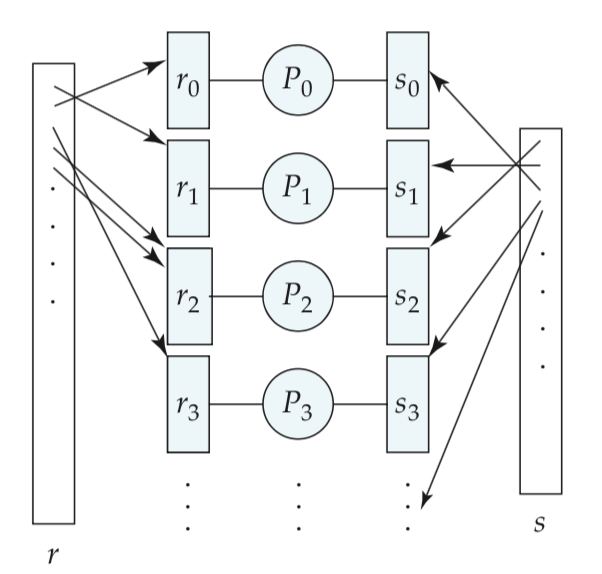
\includegraphics[width=0.3\textwidth]{images/partitioned-parallel-join}\\
Partitioned Parallel Join~\cite{dsc}.
\end{center}

Partitioning is not suitable for all types of joins, however; because we put in the restriction that there is a join on an equality condition. A more general approach is the \textit{asymmetric fragment-and-replicate join} which has three steps~\cite{dsc}:

\begin{enumerate}
\item Partition one of the relations ($r$) and hand out the partitions to the processors.
\item Send copies of the whole other relation ($s$) to every processor.
\item Each processor computers its join (through whatever method) and the data is recombined. 
\end{enumerate}

It would be preferable to choose the smaller relation to be the one that is copied as it would obviously mean less data needs to be copied to execute this algorithm.

The diagram below shows the asymmetric fragment-and-replicate join; the general case appears on the right where there are $m \times n$ processors rather than just $n$. In a typical server, the asymmetric approach is suitable. But in theory if you had a very large number of cores then you might use the general replication routine. 

\begin{center}
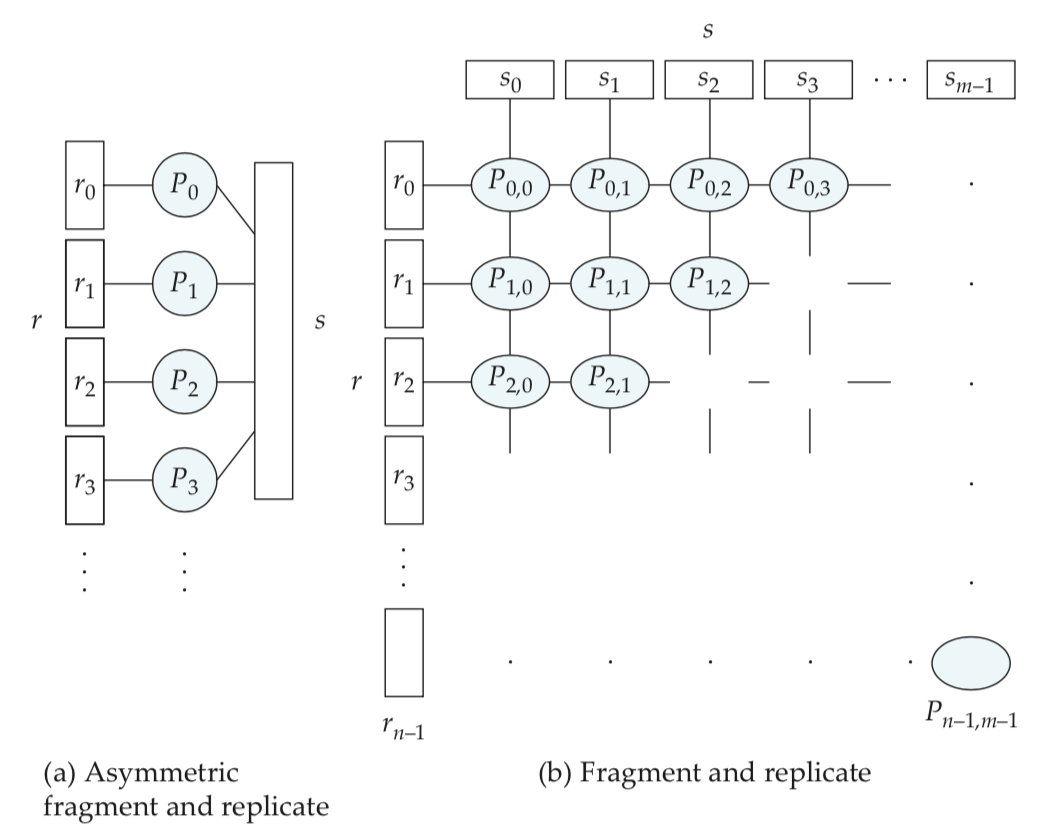
\includegraphics[width=0.7\textwidth]{images/fragment-and-replicate}\\
Fragment and Replicate~\cite{dsc}.
\end{center}

A quick rundown, then on how parallelism affects operations other than selection and join~\cite{dsc}:
\begin{itemize}
\item \textbf{Duplicate Elimination}: Duplicates are typically removed by sorting, which itself is something we could do in parallel. Also, if we partition a relation on an attribute, each processor can easily remove duplicates of that attribute.
\item \textbf{Projection}: Projection can be done as each item is read from disk; just take what you need.
\item \textbf{Aggregation}: Aggregation can be partially done locally and then the results can be combined to produce a global value. That is easy to imagine for something like sum (each processor computes its local sum, they are all added together). The same is true for count. Minimum and maximum involve comparison rather than addition to combine their values. Average, however, is more interesting: we would likely take the numerator (sum) and denominator (number of tuples) and recombine those.

\end{itemize}

\paragraph{Interoperation Parallelism.}

\bibliographystyle{alphaurl}
\bibliography{356}


\end{document}
